% LaTeX Template für Abgaben an der Universität Stuttgart
% Autor: Sandro Speth
% Bei Fragen: Sandro.Speth@studi.informatik.uni-stuttgart.de
%-----------------------------------------------------------
% Hauptmodul des Templates: Hier können andere Dateien eingebunden werden
% oder Inhalte direkt rein geschrieben werden.
% Kompiliere dieses Modul um eine PDF zu erzeugen.

% Dokumentenart. Ersetze 12pt, falls die Schriftgröße anzupassen ist.
\documentclass[12pt]{scrartcl}
% Einbinden der Pakete, des Headers und der Formatierung.
% Mit den \include und \input Befehlen können Dateien eingebunden werden:
% \include: Fügt einen Seitenumbruch nach dem Text ein
% \input: Fügt KEINEN Seitenumbruch nach dem Text ein
\input{../styles/Packages.tex}
\input{../styles/FormatAndHeader.tex}

% Counter für das Blatt und die Aufgabennummer.
% Ersetze die Nummer des Übungsblattes und die Nummer der Aufgabe
% den Anforderungen entsprechend.
% Definiert werden die Counter in FormatAndHeader.tex
% Beachte:
% \setcounter{countername}{number}: Legt den Wert des Counters fest
% \stepcounter{countername}: Erhöht den Wert des Counters um 1.
\setcounter{sheetnr}{4} % Nummer des Übungsblattes
\setcounter{exnum}{1} % Nummer der Aufgabe

\usetikzlibrary{chains,positioning}

% Beginn des eigentlichen Dokuments
\begin{document}

% Nutze den \exercise{Aufgabenname} Befehl, um eine neue Aufgabe zu beginnen.
% Möchtest du eine Aufgabe in der Nummerierung überspringen, schreibe vor der Aufgabe: \stepcounter{exnum}
% Möchtest du die Nummer einer Aufgabe auf eine beliebige Zahl x setzen, schreibe vor der Aufgabe: \setcounter{exnum}{x}
\setcounter{exnum}{1}
\exercise{IP Multicast}
    \begin{enumerate}[label=(\alph*)]
        \item \ \\
        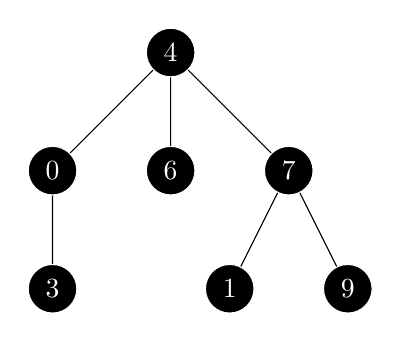
\begin{tikzpicture}[]
            \tikzset{every node/.style={draw, circle, color=white, fill=black}}

            \node {4} 
                child {
                    node {0} 
                    child { node {3} }
                    } 
                child {
                    node {6}
                    }
                child {
                    node {7} 
                        child { node {1} }
                        child { node {9} }
                    };
        \end{tikzpicture}
        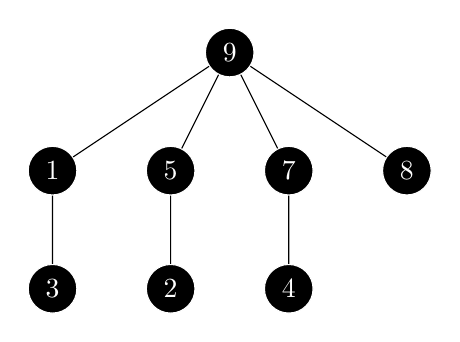
\begin{tikzpicture}
            \tikzset{every node/.style={draw, circle, color=white, fill=black}}
            \node {9}
                child { 
                    node {1}
                    child { node {3} } 
                    }
                child { 
                    node {5} 
                    child { node {2} }
                    }
                child { 
                    node {7} 
                    child { node {4} }
                    }
                child { node {8} };
        \end{tikzpicture}
        \item \ \\
            \begin{tabular}{c|c|c|c}
            Knoten & MC-Adresse & Sender & nächster Knoten \\
            \hline
            1 & MC1 & 4 & - \\
            1 & MC2 & 9 & 3 \\
            \hline
            7 & MC1 & 4 & 1, 9 \\
            7 & MC2 & 9 & 4 \\
            \hline
            \end{tabular}
    \end{enumerate}
 
\setcounter{exnum}{2}
\exercise{Traffic Shaping}
    \begin{enumerate}[label=(\alph*)]
        \item Es wurde das Leaky-Bucket Traffic-Shaping-Verfahren verwendet: Es es ist kein Burst in Abbildung b) erkennbar,
        lediglich eine konstante Obergrenze an Bytes (Abflussrate).
        \item Parameter b (Kapazität des Eimers): 2 Mb\\
        Parameter r (konstante Abflussrate): 6 Mb/s
    \end{enumerate}

\setcounter{exnum}{3}
\exercise{Queuing}
    \begin{enumerate}[label=(\alph*)]
        \item  Reihenfolge bei Fair Queuing: \\
            1, 4, 7, 9, 12, 2, 5, 8, 10, 3, 6, 11
        \item Reihenfolge bei Fair Queuing mit Byte-by-Byte-Round-Robin:\\
            12, 9, 10, 1, 7, 4, 8, 2, 11, 3, 5, 6 
        \item Reihenfolge bei Weighted Fair Queuing mit gegebenen Gewichten: \\
            12, 9, 10, 7, 8, 1, 11, 2, 3, 4, 5, 6
    \end{enumerate}

% Ende des Dokuments
\end{document}